% EmbeddingGemma 2 on African Languages
% Build: tectonic main.tex   (or: pdflatex, bibtex, pdflatex, pdflatex)
% Switch [final] to [review] for an anonymous, line-numbered ARR submission.
\documentclass[conference]{IEEEtran}
\IEEEoverridecommandlockouts
\usepackage{cite}
\usepackage{amsmath,amssymb,amsfonts}
\usepackage{graphicx}
\usepackage{booktabs}
\usepackage{multirow}
\usepackage{textcomp}
\usepackage{xcolor}
\usepackage{url}
\usepackage[T1]{fontenc}
\usepackage[utf8]{inputenc}
\usepackage{microtype}
\def\BibTeX{{\rm B\kern-.05em{\sc i\kern-.025em b}\kern-.08em T\kern-.1667em\lower.7ex\hbox{E}\kern-.125emX}}

\graphicspath{{figures/}}
\newcommand{\eg}{EmbeddingGemma}
\newcommand{\egtwo}{EmbeddingGemma~2}
\newcommand{\rone}{R@1}

\title{\eg{}~2 on African Languages: Corrected Text Benchmarks and
Speech Retrieval with a 5M-Parameter Adapter}

\author{\IEEEauthorblockN{Ugochukwu Onyebuchi}
\IEEEauthorblockA{Carnegie Mellon University / NaijaML\\
pyvinci@gmail.com}}

\begin{document}
\maketitle

\begin{abstract}
We present, to our knowledge, the first systematic evaluation of \egtwo{}, a 744M-parameter open
multimodal embedding model, on African languages. On text we re-run
AfriMTEB-Lite for both \eg{} generations and five baselines under one harness
and find that the \eg{} row in the AfriMTEB paper (29.1) does not reproduce:
under the model's intended bidirectional attention the macro score is about 45 for both generations, which share a tokenizer and score within a point of each other, and running the model with a causal instead of a
bidirectional attention mask reproduces the published macro (30.5 against 29.1 on its 12 tasks, and 35.8 against 36.0 on the seven tasks whose baselines reproduce), which we believe explains the gap. They trail a size-matched mE5-base by 12 points, more than half of it on cross-lingual bitext mining, while \egtwo{} stays within 5.5 points of 560M-parameter models on sentiment, hate-speech and emotion classification. On speech, \egtwo{} retrieves transcripts
from spoken utterances at 0.934 Recall@1 across 21 African languages zero-shot.
A LoRA adapter with 5M parameters, trained for one H100-hour on 9,000
speech--transcript pairs from six languages, raises the 14 languages it was evaluated on from 0.938 to 0.997, transfers to
seven unseen languages and to held-out sources including a language in neither
FLEURS nor the training set, matches a 1B-parameter ASR cascade in a single
pass, and, in the three languages tested at that scale, holds at 0.94--0.99 against a quarter-million candidates where the zero-shot model falls to 0.53--0.70. Cross-lingual alignment is the
model's consistent weakness: African speech retrieves English text at 0.43 and
images retrieve African-language captions at 0.17 versus 0.79 for English.
Stacking a text and an audio adapter recovers nine points of the speech-to-English gap. On
WAXAL spontaneous speech in five languages the adapter never saw, it lifts
zero-shot retrieval from 0.63 to 0.93. We release the harness, all results, the
adapter, and four tools built on it: a transcript validator, voice-note and
long-form archive search, and a cross-corpus leakage check, all running on a
4~GB laptop GPU.
\end{abstract}

\begin{IEEEkeywords}
embeddings, African languages, speech retrieval, multimodal, LoRA, benchmark reproducibility
\end{IEEEkeywords}

\section{Introduction}

\egtwo{} \cite{google2026embeddinggemma2} maps text, images, audio and video
into one 768-dimensional space and is small enough to run on a phone: 271M
parameters for text, 577M with the audio tower. That combination targets
exactly the conditions of African-language deployment, where speech often
matters more than text and connectivity is poor. Yet the model card names no
African language, and the only prior African-language benchmark result for the family, beyond a
few MMTEB tasks in its own report, is a 29.1 macro score for \eg{}~v1 \cite{vera2025embeddinggemma} in the AfriMTEB
paper \cite{uemura2026afrimteb}, with bitext and retrieval scores of 11--18 and clustering of 5 that point to an evaluation-configuration problem rather than the model's ability.

We ask three questions. (1)~What does \eg{} actually score on African text,
under the same harness as its competitors? (2)~Does the audio tower work for
African speech? (3)~Where does the shared multimodal space hold, where does it
break, and how cheaply can the breaks be repaired?

Our contributions are: a corrected AfriMTEB-Lite leaderboard with a per-task
reconciliation against the published one (\S\ref{sec:text}); to our knowledge the first speech-retrieval evaluation of \egtwo{} on African languages, with a
5M-parameter adapter that raises it to 0.997 on FLEURS, validated on held-out sources,
against an ASR cascade and at scale (\S\ref{sec:speech}); and a
characterisation of the cross-lingual failure shared by the text, speech and
vision paths (\S\ref{sec:crosslingual}).

\section{Setup}
\label{sec:setup}

\paragraph{Harness.}
\texttt{afriembed} is a single command-line interface over
sentence-transformers~6.1 \cite{reimers2019sentencebert}, transformers~5.19
and mteb~2.24 \cite{muennighoff2023mteb}. Task prompts are taken from each
model's own prompt catalog, inference is in bf16, and every result is recorded with its prompts, context cap and library versions. Results quoted without a table are in the released results files. Baselines use mteb's
registered model definitions so their published instructions are applied.

\paragraph{Text.}
AfriMTEB-Lite \cite{uemura2026afrimteb}: 13 tasks over nine languages
(Amharic, Oromo, Igbo, Yoruba, Hausa, Swahili, Kinyarwanda, Xhosa, Zulu),
comprising Flores and NTREX bitext mining \cite{nllb2022,federmann2022ntrex},
Belebele retrieval \cite{bandarkar2024belebele}, AfriXNLI
\cite{adelani2024irokobench}, MasakhaNEWS \cite{adelani2023masakhanews},
KinNews, SIB-200 classification and clustering \cite{adelani2024sib200},
Injongo intent \cite{yu2025injongo}, AfriSenti \cite{muhammad2023afrisenti},
AfriHate \cite{muhammad2025afrihate} and EmotionAnalysisPlus. We also run
AfriMTEB Full (33 text tasks, 59 languages) and CIRAL \cite{adeyemi2024ciral}
(English queries, 50k-passage pools in Hausa, Somali, Swahili, Yoruba). Two
upstream task definitions needed workarounds (an empty validation split in
EmotionAnalysisPlus; four languages missing from mteb's SIB-200 v2 dataset, the paper's SIB200\_14Classes); both
are recorded per run and applied identically to all models. Baselines are
multilingual-e5 small, base and large-instruct \cite{wang2024multilinguale5},
AfriE5 \cite{uemura2026afrimteb} and bge-m3 \cite{chen2024bgem3}.

\paragraph{Speech.}
FLEURS \cite{conneau2023fleurs} test for 21 African languages (one recording
per sentence, pools of about 300); FLEURS n-way parallel ids for cross-lingual
speech bitext; AfriSpeech-200 \cite{olatunji2023afrispeech} for accented
English; FLEURS train for fine-tuning. Held-out sources are BibleTTS
\cite{meyer2022bibletts} and NaijaVoices \cite{naijavoices2025}. Transcripts
carry the model's \texttt{document} prompt; audio carries no prompt.

\paragraph{Vision.}
Afri-Aya \cite{afriaya2025} image--caption pairs with English and
local-language captions.

\paragraph{Compute.}
About 9 H100-hours and 4 A10G-hours on Modal (\$42 at list prices),
plus a 4~GB laptop GPU for the tools.

\section{Text: the corrected benchmark}
\label{sec:text}

\begin{figure}[t]
  \centering
  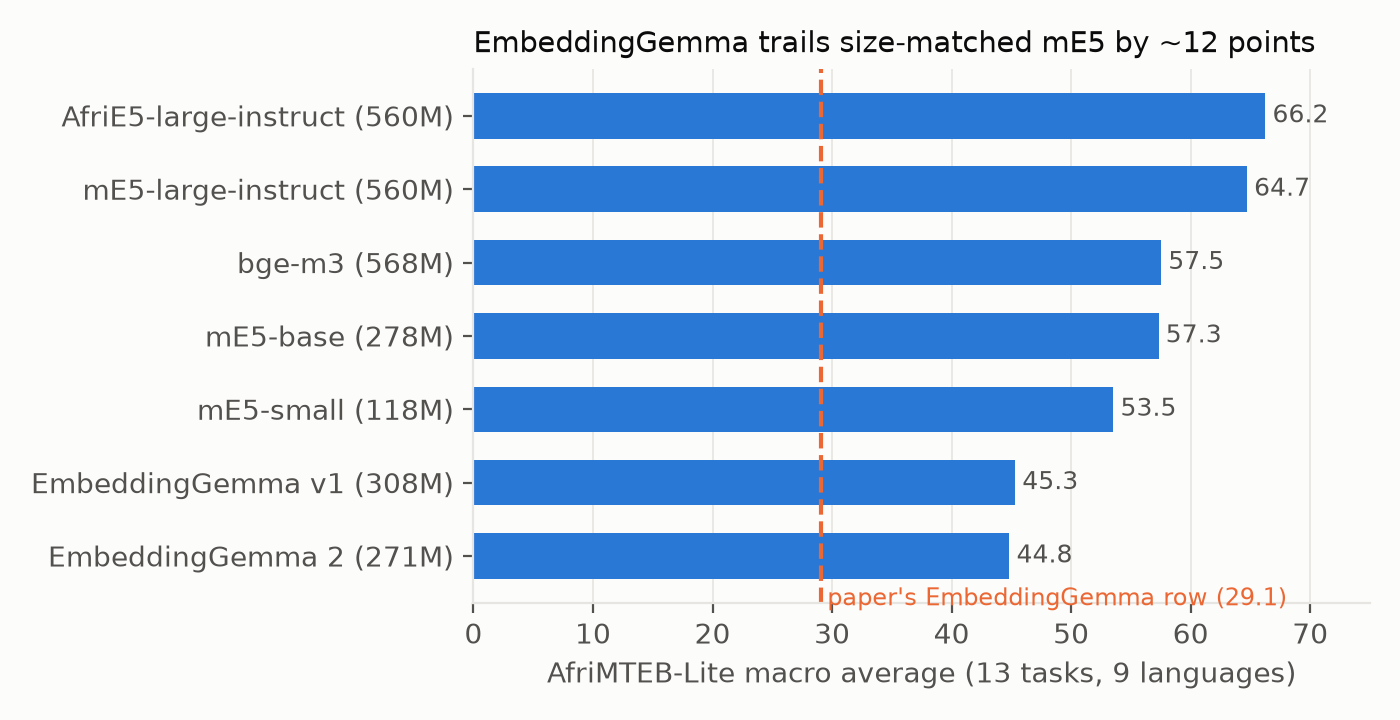
\includegraphics[width=\columnwidth]{fig1_afrimteb_lite}
  \caption{AfriMTEB-Lite macro score for seven models under one harness. Both
  \eg{} generations score about 45 on our 13-task macro (45.0 for v1 on the paper's 12 tasks), not the 29.1 published for v1.}
  \label{fig:lite}
\end{figure}

\begin{table*}[t]
  \centering
  \caption{AfriMTEB-Lite (13 tasks, 9 languages). Flores and NTREX are bitext
  F1; Belebele is nDCG@10; News is MasakhaNEWS; SIB is SIB-200 classification; the remaining columns are classification accuracy. Macro is the mean over all 13 tasks, including KinNews, SIB-200 clustering and SIB-200 v2, which are not shown. \eg{} rows are at each model's full context (2K for v1, 8K for v2), other models at a 1K-token cap (512, their maximum, for the E5 models); at 1K the \eg{} macros are 0.1 higher.}
  \label{tab:lite}
  \small
  \resizebox{\textwidth}{!}{%
  \begin{tabular}{lrrrrrrrrrrrr}
    \toprule
    Model & Params & Macro & Flores & NTREX & Belebele & AfriXNLI & News & SIB & Intent & Senti & Hate & Emotion \\
    \midrule
    AfriE5-large-instruct & 560M & \textbf{66.2} & 97.9 & 94.8 & 76.4 & 68.8 & 83.5 & 71.9 & 75.0 & 55.1 & 50.9 & 31.3 \\
    mE5-large-instruct    & 560M & 64.7 & 97.8 & 94.4 & 76.0 & 64.2 & 82.9 & 71.0 & 75.5 & 49.7 & 51.1 & 29.6 \\
    bge-m3                & 568M & 57.5 & 85.0 & 82.8 & 69.9 & 68.3 & 76.8 & 55.6 & 74.8 & 51.2 & 49.5 & 28.0 \\
    mE5-base              & 278M & 57.3 & 91.3 & 88.6 & 62.9 & 63.5 & 74.9 & 54.9 & 75.0 & 51.3 & 49.0 & 29.3 \\
    mE5-small             & 118M & 53.5 & 82.8 & 81.7 & 53.0 & 62.1 & 73.4 & 52.5 & 65.0 & 46.9 & 47.2 & 28.0 \\
    \eg{} v1              & 308M & 45.3 & 42.1 & 49.0 & 54.9 & 59.2 & 75.0 & 44.2 & 59.5 & 44.2 & 48.1 & 26.5 \\
    \egtwo{}              & 271M & 44.8 & 39.5 & 47.2 & 51.8 & 59.7 & 75.0 & 43.6 & 57.0 & 49.7 & 47.9 & 28.0 \\
    \bottomrule
  \end{tabular}}
\end{table*}

Table~\ref{tab:lite} and Figure~\ref{fig:lite} give the leaderboard. Three
results follow.

\paragraph{The published v1 score does not reproduce.}
On the paper's own 12 tasks we obtain 45.0 for v1 against the published 29.1,
with Belebele 54.9 vs 10.6, Flores 42.1 vs 12.2 and NTREX 49.0 vs 17.9.
Table~\ref{tab:reconcile} reconciles every task against the paper. Seven tasks
reproduce the paper's baseline numbers for mE5-large-instruct, AfriE5 and
bge-m3 within 1.3 points (Belebele, AfriXNLI, Injongo, SIB-200 classification
and clustering, AfriHate, and News once MasakhaNEWS and KinNews are merged as
the paper does), so for those tasks our harness matches the paper's to within 1.3 points. On those seven tasks v1 differs from the paper by $+3$ to $+44$. Three tasks (Flores, NTREX, AfriSenti) run 2--7 points higher for every baseline, and Emotion 1.4--1.9 lower, consistent with differences between the task definitions the paper used and those in mteb 2.24; the correction claim does not rest on them. Disabling task prompts costs only 1--2 points and running at the model's full 2K context moves the macro by 0.1, so neither explains the published numbers. The paper does not state the framework or library versions, prompts, precision or sequence length used to evaluate \eg{}. We
reproduce the published macro by running the model with a causal
(left-to-right) attention mask instead of its bidirectional one: the paper's
12-task macro becomes 30.5 against the published 29.1 (32.0 vs 31.6
without the non-comparable SIB-200 v2), with Flores 14.0
vs 12.2, NTREX 20.1 vs 17.9, SIB-200 classification 29.5 vs 29.6 and
AfriHate 46.4 vs 45.4 (Appendix~\ref{app:causal}). On the seven tasks whose baselines reproduce, the causal run gives 35.8 against the published 36.0; the largest per-task gaps are Injongo (41.8 vs 49.4) and Belebele (16.4 vs 10.6). EmbeddingGemma's config
enables bidirectional attention through a flag that transformers versions before 4.57 silently ignore, so the encoder runs causally with no warning. This failure
is already documented for other benchmarks \cite{mteb2025gemmaissue,st2026causalissue};
what we add is evidence that it is the likely cause of the AfriMTEB row. We have shared these findings with the AfriMTEB authors, whose own limitations section notes that some models may be sensitive to settings they did not exhaustively tune; they have not yet confirmed their original setup. Precision
(fp32 45.0; fp16 yields NaN for every input), a 128-token limit (44.1) and dropping the projection layers (under 2 points on two spot-checked tasks) come nowhere near 29.

The paper also does not say which Flores and NTREX language pairs it mines.
mteb's Lite definition mines only African--African pairs. Re-running with
English pairs included (Appendix~\ref{app:bitext}) raises every model by 1--12 points and still does not reproduce the paper's baseline bitext numbers, which
sit 2--14 points below ours under either pair set. v1 scores 42--53 on Flores
under both protocols against the published 12.2.

\begin{table}[t]
  \centering
  \caption{Our score minus the AfriMTEB paper's, per task (EG v1 is
  \eg{} v1; mE5-L is mE5-large-instruct). News merges MasakhaNEWS and KinNews over
  languages, as the paper does. The top block reproduces the paper's
  baselines within 1.3; in the bottom block every baseline moves the same way. The SIB-200 v2 task is omitted because four of its
  languages are missing upstream.}
  \label{tab:reconcile}
  \small
  \setlength{\tabcolsep}{4pt}
  \begin{tabular}{lrrrr}
    \toprule
    Task & mE5-L & AfriE5 & bge-m3 & EG v1 \\
    \midrule
    AfriHate       & $-0.4$ & $-0.8$ & $-0.6$ & $+2.7$ \\
    AfriXNLI       & $-0.3$ & $-0.2$ & $-0.4$ & $+5.6$ \\
    Belebele       & $+0.3$ & $-1.3$ & $-0.0$ & $\mathbf{+44.3}$ \\
    Injongo        & $+0.0$ & $-0.4$ & $-0.6$ & $+10.1$ \\
    SIB-200 cls.   & $-0.2$ & $-0.1$ & $+0.0$ & $+14.6$ \\
    SIB-200 clust. & $-0.2$ & $-0.0$ & $+0.1$ & $+12.0$ \\
    News           & $-0.4$ & $-0.3$ & $-0.3$ & $+10.8$ \\
    \midrule
    Emotion        & $-1.9$ & $-1.5$ & $-1.4$ & $-0.1$ \\
    AfriSenti      & $+2.7$ & $+4.4$ & $+3.3$ & $+5.2$ \\
    NTREX          & $+2.9$ & $+2.8$ & $+2.4$ & $\mathbf{+31.1}$ \\
    Flores         & $+6.4$ & $+6.7$ & $+6.9$ & $\mathbf{+29.9}$ \\
    \bottomrule
  \end{tabular}
\end{table}

\paragraph{v2 equals v1 on African text.}
44.8 vs 45.3 on Lite and 52.0 vs 52.6 on the Full suite. Tokenizer fertility
is identical to the decimal across 30 languages, and both vocabularies have 262,144 entries, indicating the tokenizer did not change between generations.

\paragraph{The gap to mE5 is concentrated.}
For \egtwo{} against mE5-base, bitext mining is 40--47 vs 89--91 and clustering 14 vs 20
(44 for mE5-large-instruct), while sentiment, hate speech and emotion are
within 5.5 points of the 560M-parameter models and news is within 2 of bge-m3.

\paragraph{Compression.}
Matryoshka truncation \cite{kusupati2022matryoshka} retains 0.99 / 0.97 /
0.90 of the macro at 512 / 256 / 128 dimensions. Trimming the vocabulary to
the 23k tokens used by the nine languages plus English removes 245~MB in bf16
but costs five macro points.

\section{Speech: zero-shot and adapted}
\label{sec:speech}

\begin{figure}[t]
  \centering
  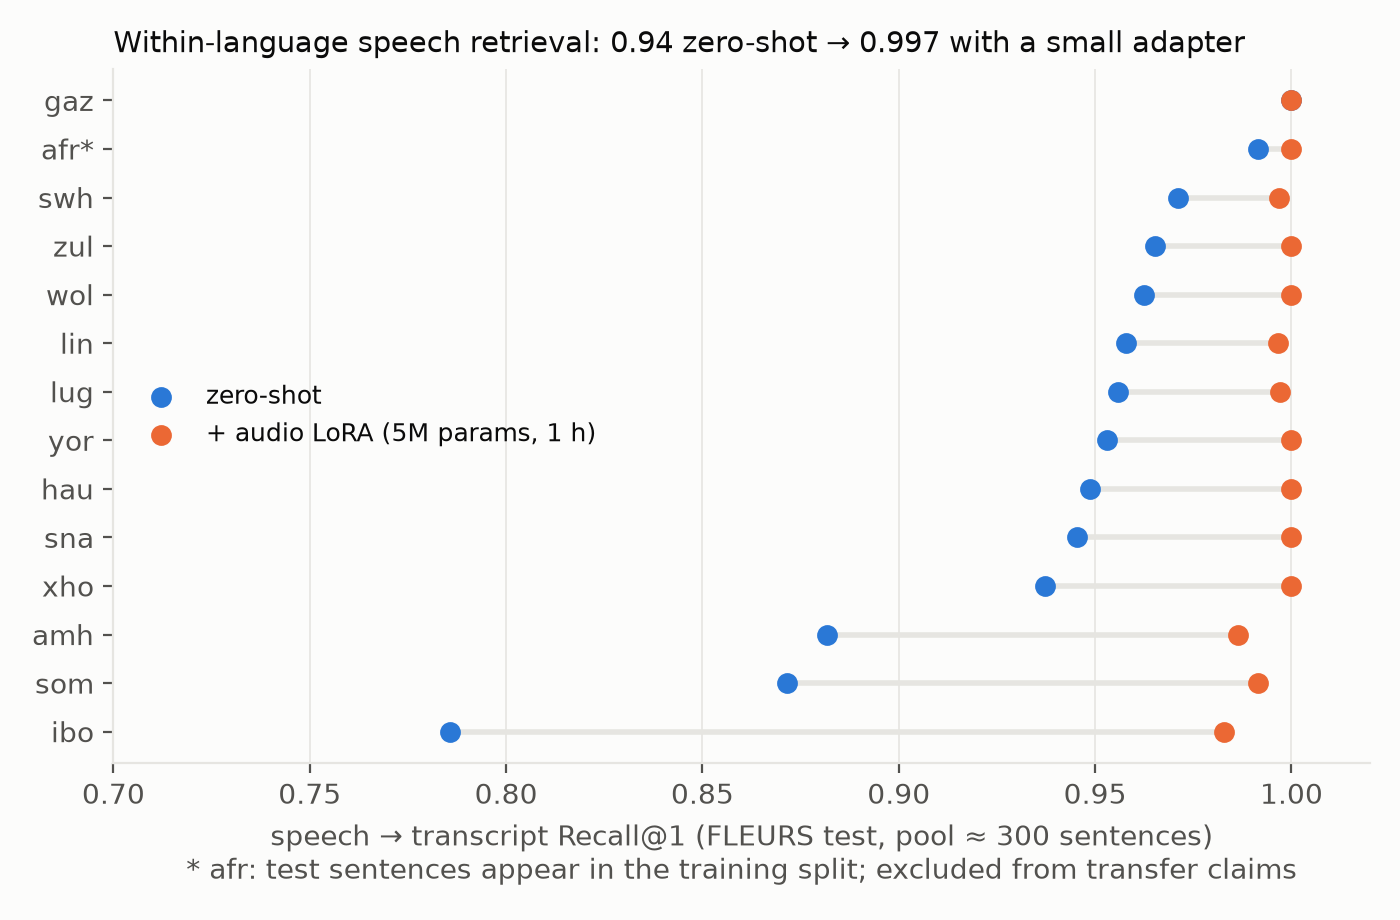
\includegraphics[width=\columnwidth]{fig2_speech_text}
  \caption{Speech-to-transcript \rone{} per language on FLEURS, zero-shot and
  with the audio adapter.}
  \label{fig:speech}
\end{figure}

\paragraph{Zero-shot.}
Speech-to-transcript \rone{} averages 0.934 over 21 languages (Figure~\ref{fig:speech} shows the 14 also evaluated with the adapter). Resource tier barely predicts the outcome (mean 0.94 for the 11 low-resource languages, 0.91 for the 7 mid and 0.97 for the 3 high): Wolof
0.962, Luo 0.974, Fulfulde 0.964 and Kabuverdianu 0.985 are low-resource, while
the weakest are Igbo 0.786, Umbundu 0.806, Somali 0.871, Kamba 0.879 and
Amharic 0.882. Removing the \texttt{document} prompt from transcripts costs up
to 23 points, most for Somali (23) and Igbo (13). On African-accented English (AfriSpeech-200, 108
accents, 1,967 utterances, full pool) \rone{} is 0.888 with no
clinical-versus-general penalty.

\paragraph{Adapter.}
We train a rank-16 LoRA \cite{hu2022lora,mangrulkar2022peft} on the text
tower's attention and MLP projections (5.0M parameters, 10~MB on disk) with a
cached contrastive loss \cite{gao2021gradcache} on 9,000 FLEURS-train
speech--transcript pairs from Hausa, Yoruba, Swahili, Amharic, Igbo and Somali
for one epoch, about one H100-hour. The mean over the 14 evaluated languages (the six training languages, the seven unseen ones below, and Afrikaans) rises from 0.938 to 0.997 (0.996 without Afrikaans); retraining with two more seeds, which change the LoRA initialisation and data order, gives 0.9964--0.9965, with 128-dimensional retention of 0.988--0.989. The LoRA sits on the text tower, which also processes the audio tower's output, so it is active for both audio and transcripts. Gains
concentrate where the base was weakest (Igbo $+20$, Amharic $+10$, Somali
$+12$) and transfer to seven languages absent from training (Xhosa, Zulu, Wolof, Luganda,
Lingala, Shona and Oromo reach 0.99--1.00; Oromo has only 36 test clips). Training and test sentences are disjoint across languages: FLEURS shares sentence ids between languages, so we checked the test sentences of all 21 languages, the six training languages included, against the 1,509 FLORES sentence ids in the training data, and found no overlap in 20 of them. The exception is Afrikaans, whose 233 test sentences all occur in the other languages' training split, so it is excluded from every transfer claim (script in the released code).
Unfreezing the 306M-parameter audio tower adds 0.001. The adapter also repairs
low-dimensional embeddings: 128-dimensional retention rises from 0.82 to 0.99
(Figure~\ref{fig:matryoshka}). Evaluating with transcripts shuffled, so that no clip is paired with its own
text, gives 0.003 for both models, exactly chance, so the metric does not leak
targets.

\begin{figure}[t]
  \centering
  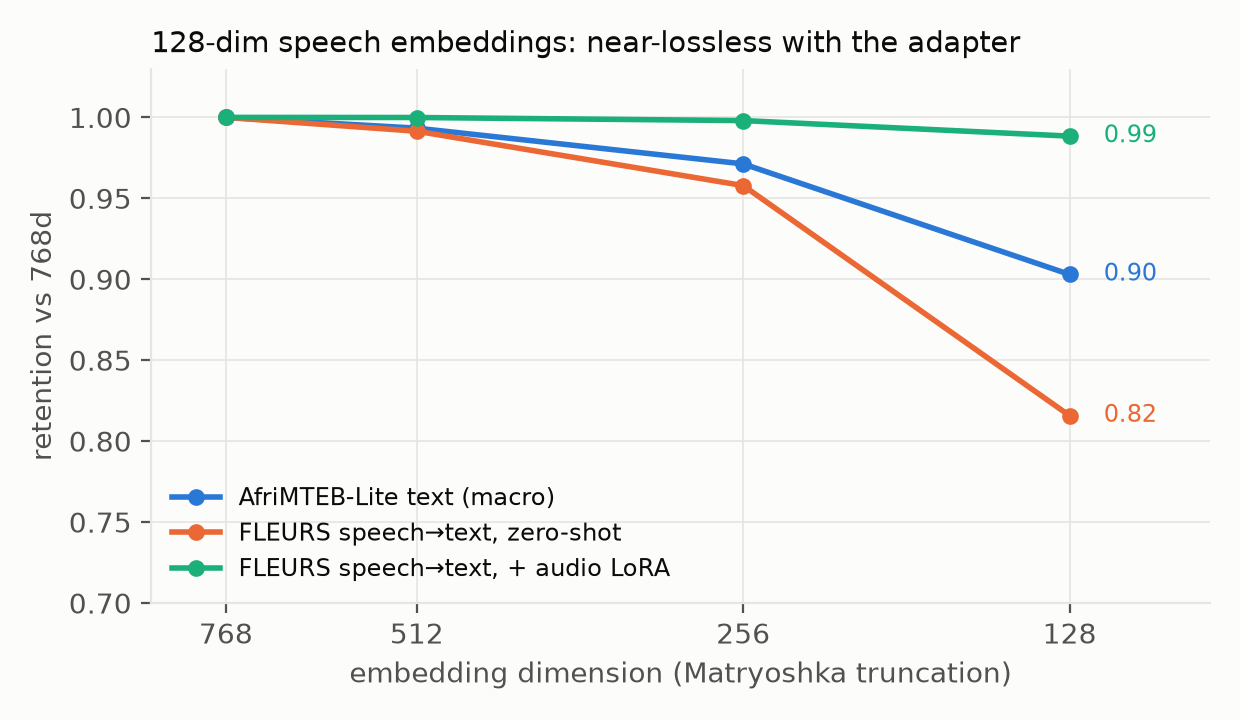
\includegraphics[width=\columnwidth]{fig3_matryoshka}
  \caption{Retention of full-dimension \rone{} under Matryoshka truncation,
  zero-shot and with the adapter.}
  \label{fig:matryoshka}
\end{figure}

\paragraph{Held-out sources.}
To reduce the risk of FLEURS leakage we evaluate on sources outside FLEURS and outside the adapter's training data (Google has not published the base model's training data) (Table~\ref{tab:heldout}, Figure~\ref{fig:heldout}): BibleTTS verses in
Hausa and in Ewe, a language in neither FLEURS nor the adapter's training set,
and NaijaVoices crowd recordings of about 3~s in Hausa, Igbo and Yoruba, with pools of 409--1,000 against about 300 on FLEURS. The zero-shot model scores
0.60--0.88 and the adapter 0.84--0.995, including 0.995 on Ewe. WAXAL
\cite{waxal2026}, released in February 2026, adds spontaneous, image-prompted speech
in five languages the adapter never saw (four of them also in FLEURS): zero-shot \rone{} is 0.49--0.76
(mean 0.63) and the adapter raises every language by 24--34 points (mean
0.93; 0.926--0.928 over three training seeds, Ewe 0.782--0.787), with Luganda, Oromo and Shona above 0.98.

\begin{table}[t]
  \centering
  \caption{Speech-to-transcript \rone{} on sources outside FLEURS. Ewe is in
  neither FLEURS nor the adapter's training languages; the five WAXAL
  languages (spontaneous image-prompted speech, 17--24~s clips) are all absent from the
  adapter's training set.}
  \label{tab:heldout}
  \small
  \begin{tabular}{llrrr}
    \toprule
    Source & Lang & Pool & Zero-shot & +LoRA \\
    \midrule
    BibleTTS    & hau & 998  & 0.861 & 0.994 \\
    BibleTTS    & ewe & 409  & 0.883 & 0.995 \\
    NaijaVoices & hau & 1000 & 0.823 & 0.959 \\
    NaijaVoices & ibo & 998  & 0.599 & 0.837 \\
    NaijaVoices & yor & 980  & 0.765 & 0.913 \\
    \midrule
    WAXAL       & lug & 600 & 0.705 & 0.995 \\
    WAXAL       & orm & 600 & 0.757 & 0.993 \\
    WAXAL       & sna & 600 & 0.645 & 0.985 \\
    WAXAL       & lin & 600 & 0.547 & 0.875 \\
    WAXAL       & ewe & 600 & 0.488 & 0.783 \\
    \bottomrule
  \end{tabular}
\end{table}

\begin{figure}[t]
  \centering
  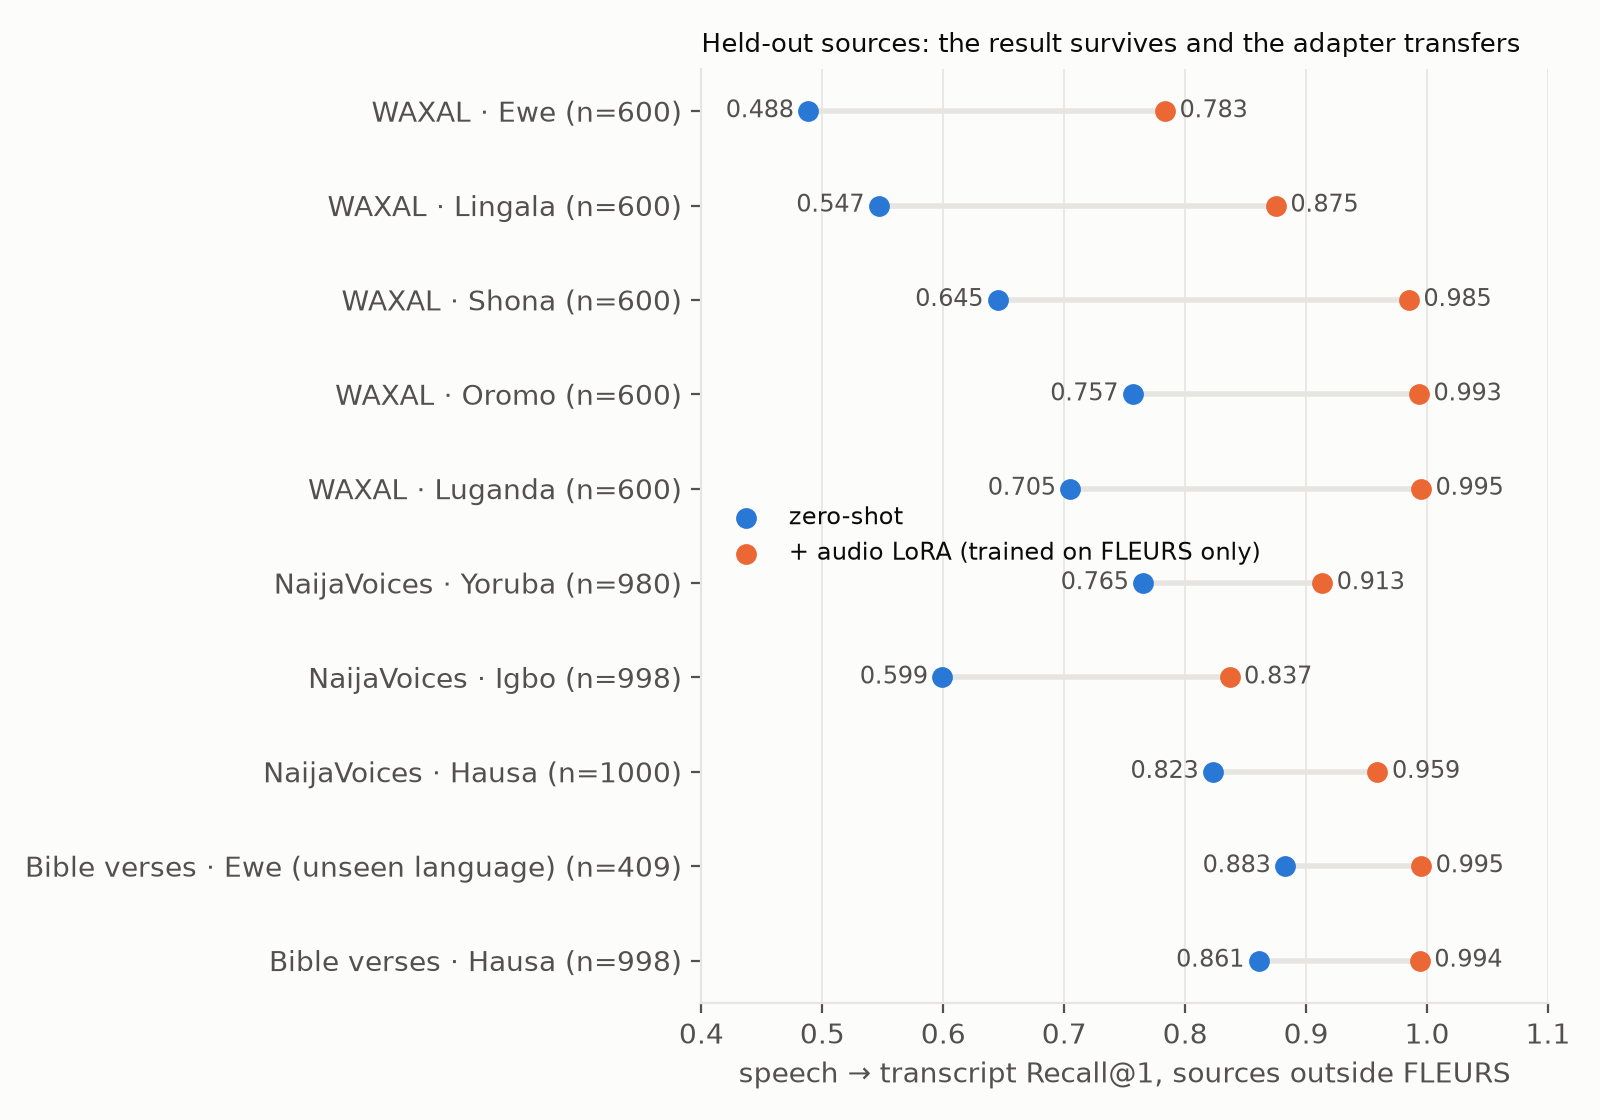
\includegraphics[width=\columnwidth]{fig5_heldout}
  \caption{Held-out sources: zero-shot versus adapted \rone{}.}
  \label{fig:heldout}
\end{figure}

\paragraph{Cascade baseline.}
The natural alternative to direct speech retrieval is a cascade: transcribe,
then embed the transcript. Table~\ref{tab:cascade} compares a cascade of
MMS-1B-all \cite{pratap2024mms} with greedy decoding and the same text
embedder against the direct path over ten languages. Retrieval from noisy
transcripts is robust even at 54\% word error rate: the cascade reaches 0.990
and beats the zero-shot direct path by 7 points on average and by 20 on Igbo.
The adapted direct path, at 0.995, matches or beats the cascade in nine of
ten languages (Amharic 0.986 against 1.000) in one pass, with no 1B-parameter recogniser and no transcription step. Its pools are the full test sets (239--350), never smaller than the cascade's, which can only lower its score.

\begin{table}[t]
  \centering
  \caption{Cascade (MMS-1B-all ASR then text embedding) versus direct
  speech retrieval, \rone{} on FLEURS pools of about 300. Direct+LoRA uses
  the full test pool per language (239--350).}
  \label{tab:cascade}
  \small
  \begin{tabular}{lrrrr}
    \toprule
    Language & WER & Cascade & Direct & Direct+LoRA \\
    \midrule
    Hausa   & 0.256 & 0.993 & 0.953 & 1.000 \\
    Yoruba  & 0.535 & 0.997 & 0.957 & 1.000 \\
    Swahili & 0.147 & 0.997 & 0.970 & 0.997 \\
    Amharic & 0.273 & 1.000 & 0.882 & 0.986 \\
    Igbo    & 0.442 & 0.977 & 0.777 & 0.983 \\
    Somali  & 0.440 & 0.980 & 0.877 & 0.991 \\
    Xhosa   & 0.370 & 0.987 & 0.943 & 1.000 \\
    Zulu    & 0.337 & 0.993 & 0.963 & 1.000 \\
    Wolof   & 0.388 & 0.996 & 0.962 & 1.000 \\
    Luganda & 0.439 & 0.983 & 0.957 & 0.997 \\
    \midrule
    Mean    & 0.363 & 0.990 & 0.924 & \textbf{0.995} \\
    \bottomrule
  \end{tabular}
\end{table}

\paragraph{Scale.}
Pools of 300 flatter any retriever. We grow the candidate set from the
queries' own transcripts to all FLEURS sentences, 50k CIRAL news passages, and
those passages split into sentences, reaching 235k--273k same-language
candidates (Table~\ref{tab:largepool}, Figure~\ref{fig:largepool}). Against the
largest pools the adapted model retrieves at 0.967 (Hausa), 0.943 (Yoruba) and
0.987 (Swahili), where the zero-shot model falls to 0.70, 0.53 and 0.70. At 256
dimensions the adapter still scores 0.953 / 0.918 / 0.967. Crowd-recorded
NaijaVoices queries at the largest pool move from 0.76 to 0.94 (Hausa) and 0.48
to 0.89 (Yoruba).

\begin{table}[t]
  \centering
  \caption{\rone{} against nested candidate pools (768 dimensions). The largest pools hold 235k--273k sentences. Queries are 300 FLEURS clips plus, for Hausa and Yoruba, about 300 NaijaVoices clips, so the smallest pool (the queries' own transcripts) holds 300--600 sentences.}
  \label{tab:largepool}
  \small
  \setlength{\tabcolsep}{4pt}
  \begin{tabular}{llrrrr}
    \toprule
    Lang & Model & 300--600 & $\sim$2k & $\sim$52k & $\sim$250k \\
    \midrule
    \multirow{2}{*}{Hausa}   & zero-shot & 0.863 & 0.860 & 0.840 & 0.700 \\
                             & +LoRA     & 0.988 & 0.988 & 0.988 & \textbf{0.967} \\
    \multirow{2}{*}{Yoruba}  & zero-shot & 0.878 & 0.832 & 0.770 & 0.530 \\
                             & +LoRA     & 0.973 & 0.973 & 0.973 & \textbf{0.943} \\
    \multirow{2}{*}{Swahili} & zero-shot & 0.970 & 0.947 & 0.867 & 0.697 \\
                             & +LoRA     & 0.997 & 0.997 & 0.990 & \textbf{0.987} \\
    \bottomrule
  \end{tabular}
\end{table}

\begin{figure*}[t]
  \centering
  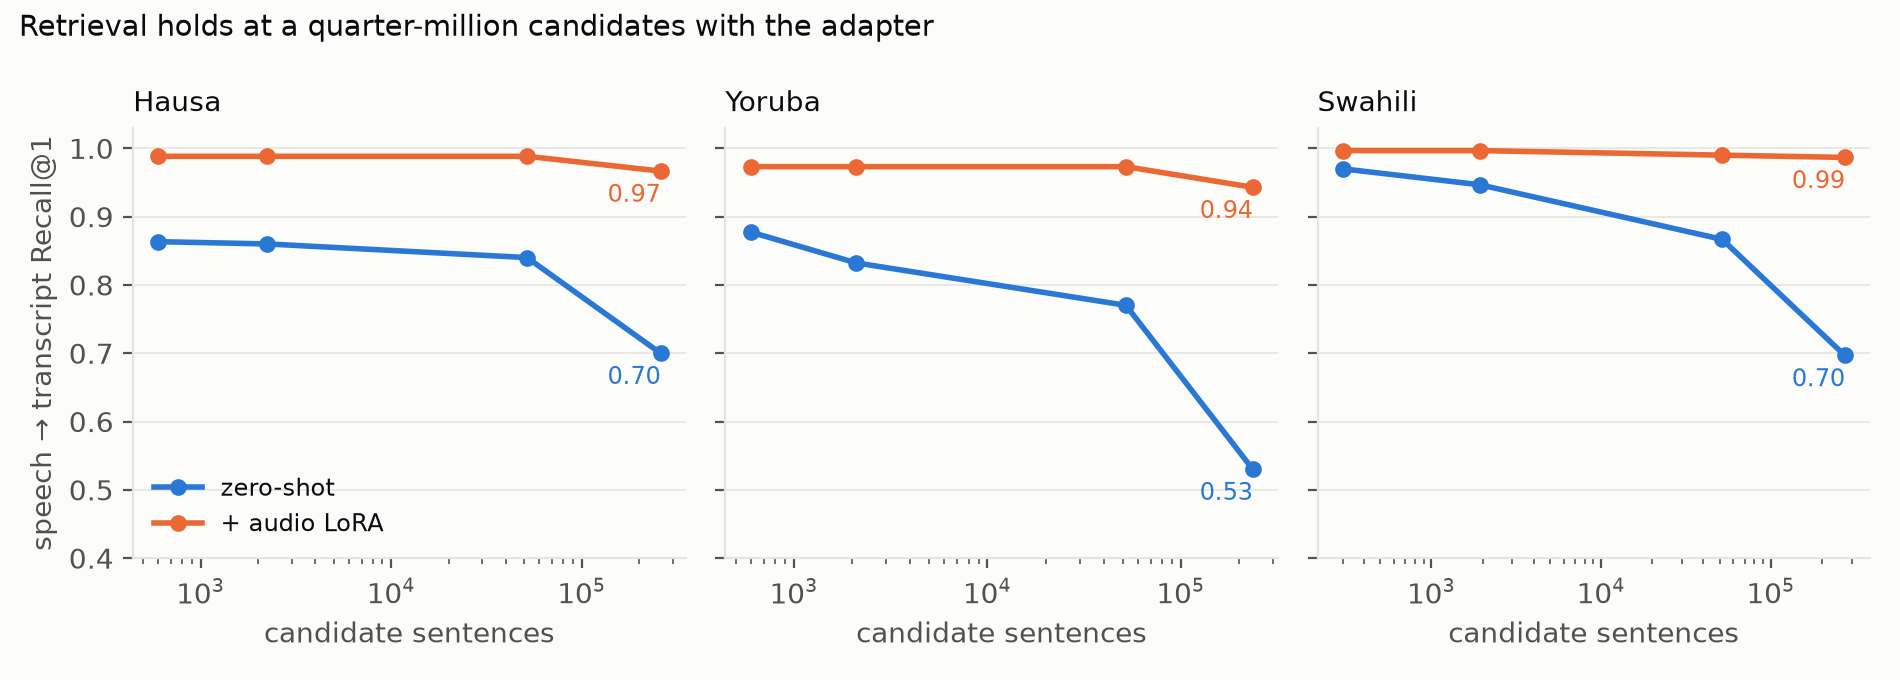
\includegraphics[width=\textwidth]{fig6_largepool}
  \caption{\rone{} against pool size for Hausa, Yoruba and Swahili, zero-shot
  and with the audio adapter.}
  \label{fig:largepool}
\end{figure*}

\section{Where the shared space breaks: cross-lingual alignment}
\label{sec:crosslingual}

\begin{figure}[t]
  \centering
  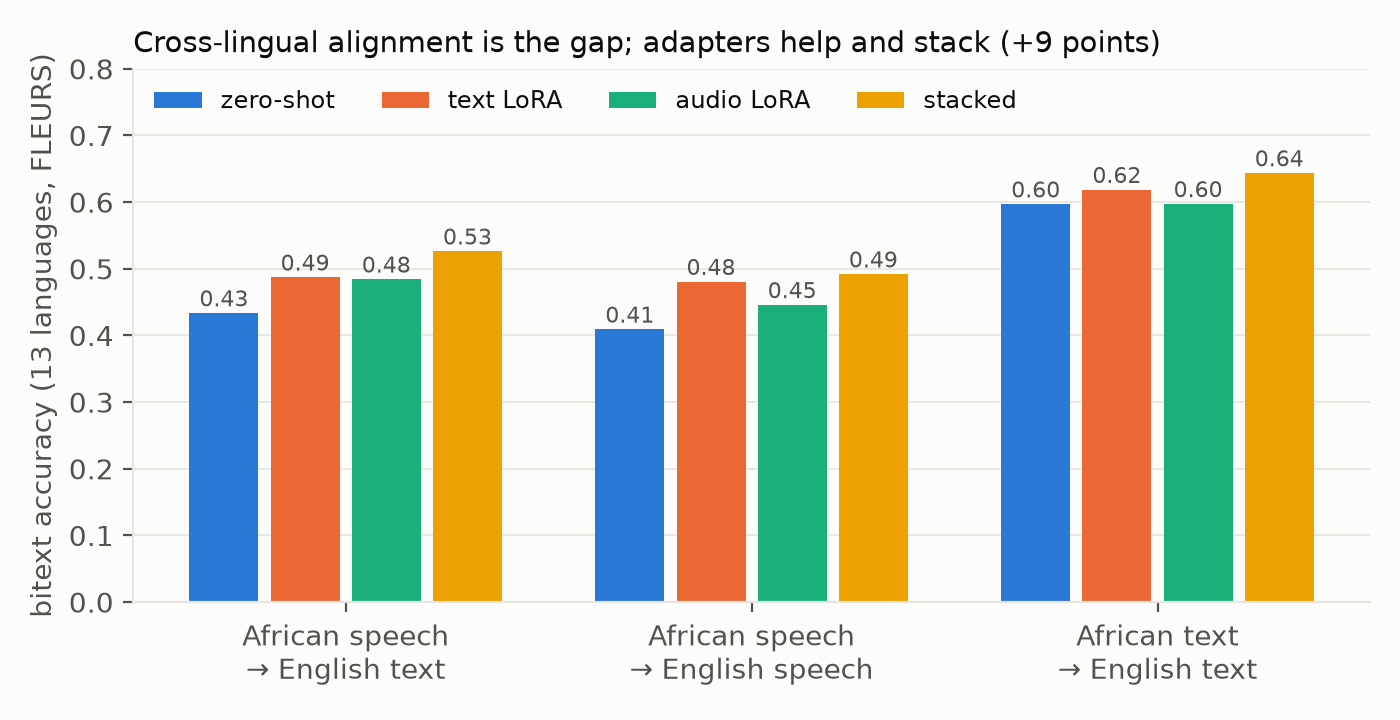
\includegraphics[width=\columnwidth]{fig4_crosslingual}
  \caption{Cross-lingual bitext \rone{}, mean over 13 African languages, for
  the zero-shot model and each adapter configuration.}
  \label{fig:crosslingual}
\end{figure}

Over 13 languages, recordings that retrieve their own transcript at 0.93 retrieve the English translation at only 0.43, and English speech at 0.41
(Figure~\ref{fig:crosslingual}). Only Swahili (0.72) and Amharic (0.63) are
well aligned; most languages sit at 0.33--0.45 and African--African pairs
average 0.34. The failure appears to lie in the text space: text-to-text bitext is 0.60 on
the same pairs, Afri-Aya images retrieve their English caption at 0.79 but
their local caption at 0.17, and local and English captions of the same image
match at only 0.07--0.19 for nine of the twelve Afri-Aya languages (the others: Igbo 0.38, Egyptian Arabic 0.96, Krio 0.84; pools of about 300). On CIRAL passage retrieval, by contrast,
\egtwo{} (0.380 nDCG@20) ties mE5-base (0.379), suggesting topical overlap suffices for passages where exact alignment does not for sentences.

Two cheap interventions each recover about five points of cross-lingual speech
retrieval (Table~\ref{tab:xling}): the audio adapter (0.434 to 0.484) and a
text-side LoRA trained on 45k caption translation pairs (0.434 to 0.487).
Activating both adapters together is nearly additive (0.526, a 9.2-point gain against 10.3 for the two separately; text-to-text 0.644), with every one of the 13 languages improving. The audio adapter leaves mean text-to-text bitext at 0.597, but per-language scores move both ways (Oromo 0.39 to 0.47, Yoruba 0.55 to 0.52). The text adapter does not improve AfriMTEB-Lite (44.9 to 44.0 at the same 1K-token context) and hurts intent classification, suggesting caption pairs are too small and too narrow a signal. A fine-tune on real parallel corpora is
the natural next step, and because audio inherits the text space, it should
lift speech cross-lingually as well.

\begin{table}[t]
  \centering
  \caption{Cross-lingual bitext \rone{} (FLEURS n-way parallel ids, 13
  languages to English) with the text LoRA, the audio LoRA, and both stacked.}
  \label{tab:xling}
  \small
  \setlength{\tabcolsep}{4pt}
  \begin{tabular}{lrrrr}
    \toprule
    Direction & Base & +text & +audio & both \\
    \midrule
    audio $\to$ English text  & 0.434 & 0.487 & 0.484 & \textbf{0.526} \\
    audio $\to$ English audio & 0.409 & 0.481 & 0.446 & \textbf{0.492} \\
    text $\to$ English text   & 0.597 & 0.619 & 0.597 & \textbf{0.644} \\
    text $\to$ English audio  & 0.554 & 0.573 & 0.546 & \textbf{0.602} \\
    \bottomrule
  \end{tabular}
\end{table}

\section{Other findings}

Spoken language identification from raw audio embeddings reaches 0.67 5-NN accuracy over 21 languages (chance 0.048), with Zulu/Xhosa the dominant
confusion. The Gemma tokenizer spends 1.95$\times$ as many tokens per word on
African languages as on English, against 1.66$\times$ for XLM-R
\cite{conneau2020xlmr} and 1.33$\times$ for NLLB-200 \cite{nllb2022}; Zulu,
Xhosa and Tigrinya cost 2.6--2.7$\times$. Fragmentation does not predict bitext quality (Pearson $r=-0.21$ against text bitext over 13 languages).

\section{Tools built on the adapter}
\label{sec:tools}

Four tools follow directly from within-language speech retrieval and run on a
4~GB laptop GPU; each is released with the harness and measured in the
results file. (1)~A \emph{transcript validator} flags clips whose audio does not
match the claimed transcript: with 10\% of labels deliberately shuffled, it
caught 251 of 251 wrong labels across NaijaVoices Hausa, BibleTTS Hausa and
WAXAL Luganda as hard fails at 0.93--1.00 precision (at most 0.9\% of clean clips failed; counting borderline clips sent for review, 1--8\% are flagged), and
surfaced a genuine label error in NaijaVoices. (2)~\emph{Voice-note search}:
a recording of a sentence retrieves another reader's recording of the same
sentence at 0.996 \rone{} over six languages (FLEURS, pools of 175--300).
(3)~\emph{Long-form archive search}: over 23 minutes of continuous Hausa
speech indexed as 10~s windows, a spoken query finds the right window at 0.81
(top-1) and 0.98 (top-3). (4)~A \emph{cross-corpus leakage check} finds
sentences of one corpus spoken in another from audio alone, with precision
1.00 and recall 0.95 on a positive control and no false positives across three
Hausa corpora. A spoken-question benchmark over English passages (Spoken
AfriQA) and ASR-free spoken intent routing (Spoken Injongo), both with
synthetic MMS-TTS queries, are also released;
the former is a negative result in the African-to-English direction (0.19
\rone{} spoken vs 0.82 typed in English; the Igbo TTS voice is largely unintelligible: its clips retrieve their own text at only 0.28 and Igbo scores 0.05), the latter reaches 0.80 accuracy over
40 intents for spoken Hausa against 0.92 typed.

\section{Limitations}

FLEURS sentence ids are shared across languages, so we checked every test
sentence in all 21 languages against the six training languages' train split:
only Afrikaans overlaps (all 233 test sentences), and it is excluded from every
transfer claim; the means move by 0.0003 (adapted) and 0.003 (zero-shot) without it.
FLEURS is public and may be in the audio encoder's training data; the held-out
evaluation on NaijaVoices and BibleTTS reduces this risk, though its pools are
still around 1,000. Most retrieval pools are small (about 300); the large-pool
test covers three languages up to 273k candidates and the others are untested
at that scale. The cascade baseline uses one recogniser with greedy decoding; a
stronger recogniser or language-model rescoring would raise it. Baselines
re-run through mteb score about 3 points above the paper on its 12-task macro,
mostly from SIB-200 v2 (four languages missing upstream) and from Flores,
NTREX and AfriSenti; rankings are unaffected, and the correction claim rests
only on the seven tasks whose baselines reproduce. The AfriMTEB paper's bitext protocol could not be recovered from its
text, so its bitext columns are compared under two pair sets rather than one.
Two AfriMTEB-Lite languages (Kinyarwanda, Oromo) have little or no FLEURS
audio. The adapter was trained with three seeds; every other result comes from a single run.

\section{Conclusion}

\egtwo{} is a weak cross-lingual aligner for African languages and a middling within-language text embedder, but its audio tower works for African speech out of the box. For on-device voice search in a single language the zero-shot model
is usable but is beaten by a conventional recogniser-plus-embedder cascade; a
10~MB adapter closes that gap in a single pass, is near-perfect on FLEURS, including seven languages it never saw, reaches 0.78--0.995 on held-out recordings, and, in the three languages tested, holds up at indexes of a quarter-million sentences. Cross-lingual use needs a real parallel-data fine-tune, which the stacking result suggests will carry over to speech.

\section*{Artifacts}

The harness, raw per-run results with prompts, versions and caveats, and all
figures are released with the paper. The audio adapter is available at
\url{https://huggingface.co/naijaml/embeddinggemma-2-african-speech-lora}.

\appendices

\section{Bitext mining with English pairs}
\label{app:bitext}

mteb's AfriMTEB-Lite definition mines the 72 African--African Flores pairs among the nine Lite languages and 30 NTREX pairs among the six it covers, with no English (Kinyarwanda appears in NTREX only paired with English). The AfriMTEB
paper does not state which pairs it mines. Table~\ref{tab:bitext-eng} reruns
both tasks with English pairs (18 for Flores, 14 for NTREX).

\begin{table}[t]
  \centering
  \caption{Bitext F1 with English--African pairs (eng) and African--African
  pairs (Afr) against the AfriMTEB paper's figures. The Afr columns come from this rerun and differ from Table~\ref{tab:lite} by at most 0.1.}
  \label{tab:bitext-eng}
  \small
  \setlength{\tabcolsep}{3pt}
  \resizebox{\columnwidth}{!}{%
  \begin{tabular}{lrrrrrr}
    \toprule
    & \multicolumn{2}{c}{Flores} & \multicolumn{2}{c}{NTREX} & \multicolumn{2}{c}{Paper} \\
    \cmidrule(lr){2-3}\cmidrule(lr){4-5}\cmidrule(lr){6-7}
    Model & eng & Afr & eng & Afr & Flores & NTREX \\
    \midrule
    \eg{} v1 & 53.2 & 42.2 & 52.5 & 49.0 & 12.2 & 17.9 \\
    \egtwo{} & 51.4 & 39.5 & 49.6 & 47.2 & --   & --   \\
    mE5-large-instruct & 99.2 & 97.9 & 98.1 & 94.3 & 91.4 & 91.5 \\
    AfriE5   & 99.3 & 97.9 & 98.1 & 94.8 & 91.2 & 92.0 \\
    bge-m3   & 91.6 & 85.0 & 88.9 & 82.8 & 78.1 & 80.4 \\
    \bottomrule
  \end{tabular}}
\end{table}

English pairs score higher than African--African pairs for every model, and
neither pair set reproduces the paper's baseline bitext numbers.

\section{Reproducing the published score}
\label{app:causal}

EmbeddingGemma v1 on AfriMTEB-Lite under the same harness, with its
bidirectional attention (correct) and with a causal mask, against the AfriMTEB
paper's published row.

\begin{table}[t]
  \centering
  \small
  \setlength{\tabcolsep}{4pt}
  \caption{EmbeddingGemma v1 with correct (bidirectional) and causal attention against the AfriMTEB paper's row.}
  \label{tab:causal}
  \begin{tabular}{lrrr}
    \toprule
    Task & Correct & Causal & Paper \\
    \midrule
    SIB-200 cls.   & 44.2 & 29.5 & 29.6 \\
    AfriHate       & 48.1 & 46.4 & 45.4 \\
    Emotion        & 26.5 & 24.8 & 26.6 \\
    AfriXNLI       & 59.2 & 55.6 & 53.6 \\
    SIB-200 clust. & 16.6 &  3.4 &  4.6 \\
    Flores         & 42.1 & 14.0 & 12.2 \\
    NTREX          & 49.0 & 20.1 & 17.9 \\
    Belebele       & 54.9 & 16.4 & 10.6 \\
    Injongo        & 59.5 & 41.8 & 49.4 \\
    News$^\ddagger$ & 69.8 & 57.2 & 59.0 \\
    SIB-200 v2$^\dagger$ & 26.2 & 14.2 & 1.4 \\
    AfriSenti      & 44.2 & 43.0 & 39.0 \\
    \midrule
    Macro (12 tasks) & \textbf{45.0} & \textbf{30.5} & \textbf{29.1} \\
    Macro (11, no v2) & 46.7 & 32.0 & 31.6 \\
    \bottomrule
  \end{tabular}
  
\end{table}

Under a causal mask, sentiment, hate-speech, emotion and NLI lose only 1--4 points, topic and intent classification lose 13--18, and bitext, retrieval and clustering collapse by 13--39, which is the shape of the published row. The Correct column is the full-context run used throughout; the causal run used a 1K-token cap, at which the correct model gives News 70.0 and a 12-task macro of 45.1, so the cap does not affect the comparison. $^\ddagger$MasakhaNEWS and KinNews merged and averaged over
languages, as the paper does. $^\dagger$Not comparable: mteb's current
SIB-200 v2 (the paper's SIB200\_14Classes) lacks four Lite languages and every baseline runs about 25 points above the paper on it. AfriSenti runs 4 points above the paper here, as it does (3--4 points) for every baseline (Table~\ref{tab:reconcile}).

\section{Aggregating the paper's way}
\label{app:agg}

The paper's AfriMTEB-Lite is 12 tasks: MasakhaNEWS and KinNews are one News
task, and its SIB-200 task covers all nine Lite languages. Table~\ref{tab:agg}
re-aggregates our runs under that scheme and with the incomparable SIB-200 v2
task dropped. Merging the news tasks moves every macro by under 0.5; dropping SIB-200 v2 raises each by a further 1.3--2.1.

\begin{table}[t]
  \centering
  \caption{Macro scores under three aggregations (our 13 tasks; the paper's
  12 with news merged; 11 with SIB-200 v2 dropped) and the paper's published
  figures.}
  \label{tab:agg}
  \small
  \setlength{\tabcolsep}{4pt}
  \begin{tabular}{lrrrr}
    \toprule
    Model & 13 & 12 (paper) & 11 & Paper \\
    \midrule
    \eg{} v1 & 45.3 & 45.0 & 46.7 & 29.1 \\
    \egtwo{} & 44.8 & 44.4 & 46.2 & -- \\
    mE5-large-instruct & 64.7 & 65.0 & 66.5 & 62.0 \\
    AfriE5 & 66.2 & 66.6 & 67.9 & 63.7 \\
    bge-m3 & 57.5 & 57.8 & 59.9 & 55.0 \\
    \bottomrule
  \end{tabular}
\end{table}

\section{Adapter training details}
\label{app:train}

LoRA rank 16, alpha 32, no dropout, applied to the query, key, value, output,
gate, up and down projections of the text tower only (5.0M trainable
parameters, PEFT 0.21). Cached multiple-negatives ranking loss on the
768-dimensional embedding, batch size 32, learning rate $2\times10^{-5}$ with
10\% warmup, one epoch over 9,000 FLEURS-train pairs from Hausa, Yoruba,
Swahili, Amharic, Igbo and Somali, bf16, one H100 (sentence-transformers 6.1,
transformers 5.19). The adapter is loaded with sentence-transformers'
\texttt{load\_adapter} and is 10~MB on disk. Evaluating with shuffled
transcripts gives 0.003 \rone{}, exactly chance.

\bibliographystyle{IEEEtran}
\bibliography{references}

\end{document}
